\documentclass[PhD-Yoann-Dupont.tex]{subfiles}
\begin{document}

Dans le cadre de l'apprentissage statistique, deux types de modèles sont généralement utilisés : les modèles dits \emph{génératifs} et les modèles dit \emph{discriminants} \citep{ng2002discriminative}. La différence entre ces deux types de modèles est dans la loi de probabilité qu'ils modélisent. Tandis que les modèles génératifs modélisent une probabilité jointe :

\begin{equation}\label{eq:generative-equation}
p_{g} = p_{g}(y,x;\theta) = p_{g}(y|x;\theta)p_{g}(x;\theta)
\end{equation}

les modèles discriminants modélisent une probabilité conditionnelle :

\begin{equation}\label{eq:discriminative-equation}
p_{d} = p_{d}(y|x;\theta)
\end{equation}

Où $\theta$ représente les paramètres des différents modèles. Nous remarquons des formules \ref{eq:generative-equation} et \ref{eq:discriminative-equation} qu'il est possible d'établir des équivalences entre certains modèles génératifs et discriminants, certaines d'entre elles étant d'ailleurs illustrées dans la figure \ref{fig:generative-vs-discriminative}. Les modèles génératifs utilisent la probabilité de l'entrée $p(x)$, ce qui leur permet de générer de nouvelles séquences. Les modèles discriminants, quant à eux, ne modélisent qu'une probabilité conditionnelle, c'est-à-dire la probabilité d'une sortie sachant une entrée, ils ne peuvent pas générer de nouvelles séquences mais sont très efficaces pour trouver les traits distinctifs des différentes sorties possibles. Dans le cadre de l'apprentissage supervisé où l'ensemble de sortie est connu à l'apprentissage, le calcul de $p(x)$ n'est pas nécessaire voire encombrant car $x$ est toujours donnén, en plus des difficultés de paramétrage et de généralisation à des données inconnues que cela engendre.

\begin{figure}[ht!]
\centering
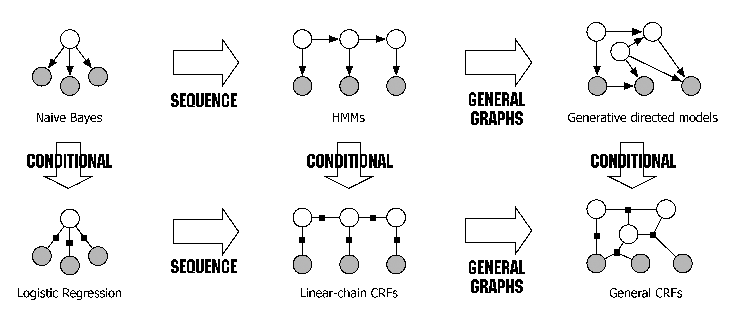
\includegraphics[scale=1.2]{images/general/generative-vs-discriminative}
\caption{quelques correspondances entre des modèles génératifs (en haut) et discriminants (en bas). Illustration faite par \citet{sutton2010introduction}}
\label{fig:generative-vs-discriminative}
\end{figure}

\end{document}